%----------------------------------------------------------------------------------------
%	PACKAGES AND THEMES
%----------------------------------------------------------------------------------------

\documentclass[presentation,aspectratio=169]{beamer}
\usepackage{graphicx} % Allows including images
\usepackage{booktabs} % Allows the use of \toprule,
\usepackage{caption}
\usepackage{subcaption}
\usepackage{amsmath}
\usepackage{mathtools, bm}
\usepackage{multicol}
% --------------------Chinese Support--------------------------
\usepackage{ctex}
\usepackage{xeCJK}
\usepackage{fontspec} 
\setCJKmainfont{Microsoft YaHei}
% --------------------Biber Support----------------------------
\usepackage[backend=bibtex]{biblatex}

\makeatletter
\let\@@magyar@captionfix\relax
\makeatother

\usefonttheme{professionalfonts}

\DeclareOptionBeamer{width}
{\PassOptionsToPackage{width=#1}{beamerouterthemesidebar}}

\DeclareOptionBeamer{hideothersubsections}
{\PassOptionsToPackage{hideothersubsections=#1}{beamerouterthemesidebar}}

\DeclareOptionBeamer{hideallsubsections}
{\PassOptionsToPackage{hideallsubsections=#1}{beamerouterthemesidebar}}

\ProcessOptionsBeamer

\mode<presentation>

\useoutertheme[height=0pt,left,hideothersubsections]{sidebar}

\usecolortheme{seahorse}
\setbeamercolor*{titlelike}{parent=structure}

\useinnertheme{rectangles}
\setbeamertemplate{frametitle}{
\leftskip=10pt\vspace{16pt}\insertframetitle
}

% ---------------Global Color Settings----------------------------
%\definecolor{xmucolor}{RGB}{0 114 198}%Blue
\definecolor{xmucolor}{RGB}{18 64 102}%XMUBlue
%\definecolor{xmucolor}{RGB}{1 168 156}%Cyan
%\definecolor{xmucolor}{RGB}{0 128 0}%Green
%\definecolor{xmucolor}{RGB}{249 105 14}%Orange
%\definecolor{xmucolor}{RGB}{102 51 153}%Purple
%\definecolor{xmucolor}{RGB}{150 40 26}%Red
% ----------------------------------------------------------------

\setbeamercolor{sidebar}{bg=xmucolor}

\setbeamercolor{author in sidebar}{bg=white,fg=white!20}
\setbeamerfont{author in sidebar}{series=\itshape}

\setbeamerfont{title}{size = {\fontsize{26}{36}}, series=\bfseries}
\setbeamerfont{author}{size = {\fontsize{20}{40}}}
\setbeamerfont{institute}{size = {\fontsize{15}{40}}}
\setbeamerfont{date}{size = {\fontsize{18}{20}}}
\setbeamerfont{frametitle}{size = {\fontsize{20}{20}}, series=\bfseries}


\setbeamercolor{title in sidebar}{bg=white,fg=white}
\setbeamerfont{title in sidebar}{series=\bfseries}

\setbeamercolor{structure}{fg=xmucolor}
\setbeamercolor{section in sidebar}{fg=white}
\setbeamercolor{subsection in sidebar}{fg=white}


\setbeamercolor{section in toc}{fg=xmucolor}
\setbeamercolor{subsection in toc}{fg=xmucolor}
\setbeamerfont{section in toc}{size = {\fontsize{16}{30}}}
\setbeamerfont{subsection in toc}{size = {\fontsize{12}{16}}}

\setbeamertemplate{section in toc}
{\leavevmode\leftskip=5ex%
	\llap{%
		\usebeamerfont*{section number projected}%
		\usebeamercolor{section number projected}%
		\begin{pgfpicture}{-1ex}{-0.5ex}{3ex}{4ex}
			\color{bg}
			\pgfpathcircle{\pgfpoint{0pt}{.75ex}}{1.7ex}
			\pgfusepath{fill}
			\pgftext[base]{\color{fg}\inserttocsectionnumber}
		\end{pgfpicture}\kern1.25ex%
	}%
	\inserttocsection\par}
\setbeamertemplate{subsection in toc}
{\leavevmode\leftskip=3em$\bullet$\hskip.5em\inserttocsubsection\par}


\setbeamerfont{caption name}{size = {\fontsize{12}{12}}}
\setbeamerfont{caption}{size = {\fontsize{12}{12}}}

%\usepackage[T1]{fontenc}
%\usepackage[default, osfigures]{opensans}

\usepackage{transparent}
\usebackgroundtemplate{
	% ---------------------aspectratio=1610-----------------------
	% \hspace*{0.235\paperwidth}
	% {
\includegraphics[width=0.6\paperwidth]{xmuese}}
	% ------------------------------------------------------------

	% ---------------------aspectratio=169------------------------
	\hspace*{0.26\paperwidth}
	{
\includegraphics[width=0.55\paperwidth]{xmuese}}
	% ------------------------------------------------------------

	% ---------------------aspectratio=43-------------------------
	%\hspace*{0.18\paperwidth}
	%{
\includegraphics[width=0.725\paperwidth]{xmuese}}
	% ------------------------------------------------------------
}

\setbeamertemplate{itemize item}[circle]
\setbeamertemplate{itemize subitem}[circle]
\setbeamertemplate{enumerate item}[circle]
\setbeamertemplate{enumerate subitem}[circle]
\setbeamercolor{block title}{bg=xmucolor,fg=white}
\setbeamercolor{block title example}{fg=xmucolor}

\makeatletter
\setbeamercolor{myfootlinetext}{fg=xmucolor}
\newdimen\mywidth%
\setlength{\mywidth}{\paperwidth}%
\addtolength{\mywidth}{-\beamer@sidebarwidth}%
\setbeamertemplate{footline}
{
  \leavevmode%
  \hbox{%
  \begin{beamercolorbox}[wd=\beamer@sidebarwidth,ht=1ex,dp=1ex,right]{sidebar}%
  \end{beamercolorbox}
  \begin{beamercolorbox}[wd=\mywidth,ht=1ex,dp=1ex,right]{myfootlinetext}%
    \usebeamerfont{date in head/foot}\hfill\insertshorttitle\hspace*{2em}\insertshortauthor{}\hspace*{2em}
    \insertframenumber{} / \inserttotalframenumber\hspace*{2ex}
  \end{beamercolorbox}}%
  \vskip0pt%
}
\makeatother

\makeatletter
\setbeamertemplate{sidebar \beamer@sidebarside}%{sidebar theme}
{
  \beamer@tempdim=\beamer@sidebarwidth%
  \advance\beamer@tempdim by -6pt%

  \vspace{0.5cm}
  \hspace{0.132cm}
\includegraphics[width=1.3cm]{xmu.pdf}
  \vspace{0.5cm}

  \insertverticalnavigation{\beamer@sidebarwidth}%
  \vfill
  \ifx\beamer@sidebarside\beamer@lefttext%
  \else%
	\usebeamercolor{normal text}%
	\llap{\usebeamertemplate***{navigation symbols}\hskip0.1cm}%
	\vskip2pt%
  \fi%
}%

\setbeamertemplate{section in sidebar}{\vbox{
	\vskip5ex
    \beamer@sidebarformat{3pt}{section in sidebar}{\insertsectionhead}}}
\setbeamertemplate{section in sidebar shaded}{\vbox{
	\vskip5ex
    \beamer@sidebarformat{3pt}{section in sidebar shaded}{\insertsectionhead}}}
\makeatother

\setbeamertemplate{navigation symbols}{} % To remove the navigation symbols from the bottom of all slides uncomment this line

\definecolor{MyBackground}{RGB}{255,241,167}
\setbeamercolor{background canvas}{bg=MyBackground}

\mode
<all>


\usepackage{listings}

\addbibresource{../paper/ref.bib}

\title[基于RISC-V指令集的通用处理器安全性研究]{基于RISC-V指令集的通用\\处理器安全性研究}
% \subtitle{————看不见我}

\author[韩博阳]{答辩人:韩博阳} % Your name
\institute[XMU]{指导老师:周剑扬}% Your instructor
\date{2022年5月19日} % Date, can be changed to a custom date

\begin{document}

\begin{frame}
\titlepage % Print the title page as the first slide
\end{frame}

\begin{frame}
\frametitle{目录} % Table of contents slide, comment this block out to remove it
    \begin{columns}[T]

        \begin{column}{.45\textwidth}
                \centering
                \tableofcontents[sections={1-2}]
        \end{column}
        \begin{column}{.45\textwidth}
                \centering
            \tableofcontents[sections={3-4}]
        \end{column}
    \end{columns}
\end{frame}



\section{研究简介}

\begin{frame}{}
    \centering
        \Huge\bfseries
    \textcolor{xmucolor}{研究简介}\\
\end{frame}

\subsection{研究背景}
\begin{frame}
\frametitle{研究背景}
\begin{figure}[ht]
    \centering
    \includegraphics[scale=0.65, page=1]{../paper/figs/figs.pdf}
    \caption{云计算平台架构}
\end{figure}
\end{frame}

\subsection{研究目标}
\begin{frame}
\frametitle{研究目标}
\begin{block}{温故}
    对近期提出的针对处理器及其系统的硬件攻击方案进行调研。
\end{block}
\begin{block}{知新}
    在RISC-V指令集硬件生态中的重要硬件产品上实现针对硬件的攻击:
    \begin{itemize}
        \item 中科院计算所的香山高性能开源处理器:针对处理器微架构的攻击;
        \item SiFive公司的HiFive Unmatched单板计算机:针对处理器系统的攻击。
    \end{itemize}
\end{block}
\end{frame}



\section{微架构攻击}

\begin{frame}{}
    \centering
    \Huge\bfseries\textcolor{xmucolor}{针对处理器微架构的攻击}\\
    \vspace{1em}
    \large\bfseries\textcolor{xmucolor}{基于预测式执行和缓存侧信道的任意地址读取}
\end{frame}

\subsection{攻击原理}
\begin{frame}[fragile]
\frametitle{攻击原理}
\begin{columns}[c]

    \column{.4\textwidth}
    \only<1>{高性能处理器广泛采用预测式乱序执行机制,以及存储器分层的设计理念。}
    \only<2>{x $\gets 2$}
    \begin{onlyenv}<1-2>
    
    \begin{lstlisting}[language=c]
if (x < a1_length) {
    result = a2[a1[x]];
}
    \end{lstlisting}
    \end{onlyenv}

    \only<3>{
        逐个测试a2中元素的读取时间,
        读取用时最短的元素对应的下标即为secret的值
    }

    \column{.6\textwidth}
    
    \only<1-2>{\begin{figure}[ht]
        \centering\includegraphics[scale=1, page=1]{./figs/figs.pdf}
    \end{figure}}

    \only<3>{\begin{figure}[ht]
        \centering\includegraphics[scale=1, page=2]{./figs/figs.pdf}
    \end{figure}}

\end{columns}
\end{frame}

\subsection{攻击实现}
\begin{frame}
\frametitle{创新算法}
\begin{block}{高速缓存控制算法}
    由于香山处理器没有提供从高速缓存中换出特定地址的直接实现方案。
    考虑到从存储器地址空间中的地址到高速缓存行之间是多对一的映射关系,
    设计了基于Evict的高速缓存控制算法,通过访问与需要被换出的地址映射
    到相同缓存行的其他地址,将其他地址换入高速缓存,替换掉需要被换出的地址。
\end{block}
\begin{block}{分支预测器训练算法}
    因为分支预测器除了会考量当前分支指令的历史(Local History,局部历史),
    也会根据最近执行过的其他分支指令的跳转方向(全局历史,Global History)做出预测。
    所以在训练分支预测器的过程中需要采用专门设计的“无分支参数选择”算法。
\end{block}
\end{frame}

\begin{frame}
\frametitle{香山RTL仿真器测试结果}
测试代码见论文附录A,在不直接访问的情况下读出secret的值(测试样例中为ASCII字母'G'):
\begin{figure}[ht]
    \centering
    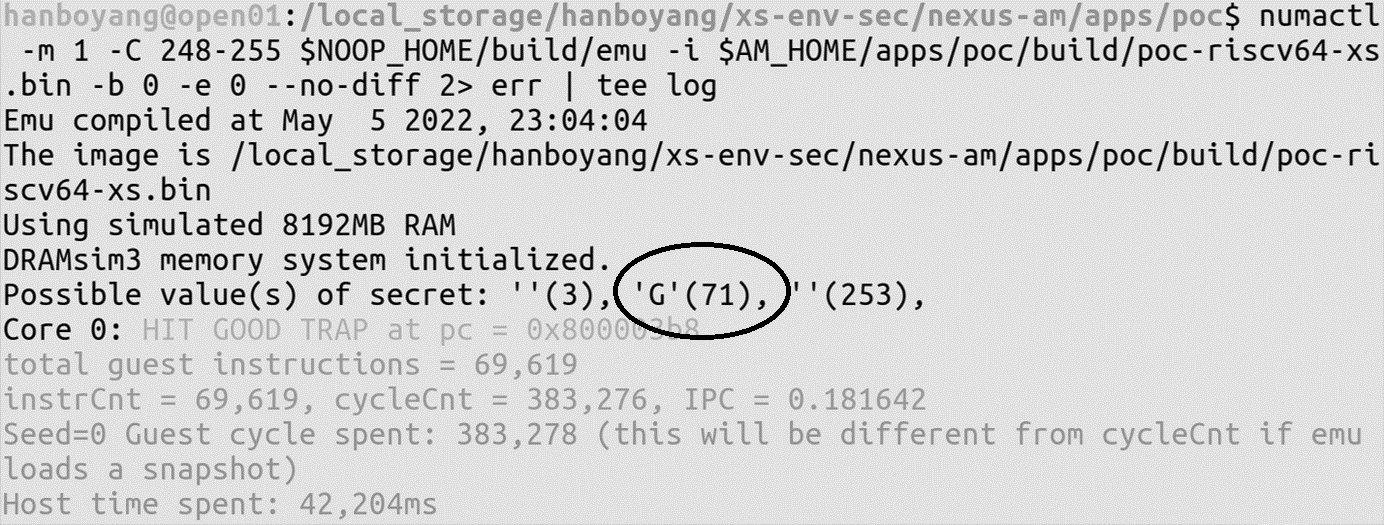
\includegraphics[width=\textwidth]{../paper/figs/spectre-result.png}
\end{figure}
\end{frame}



\section{系统攻击}

\begin{frame}{}
    \centering
    \Huge\bfseries\textcolor{xmucolor}{针对处理器系统的攻击}\\
    \vspace{1em}
    \large\bfseries\textcolor{xmucolor}{基于PCIe DMA的任意地址读取}
\end{frame}

\subsection{攻击原理}
\begin{frame}
\frametitle{处理器系统结构}
现代计算机的处理器系统一般包括以下几个基本组件:
\begin{itemize}
    \item 处理器核集合体:包括处理器核、一级高速缓存、中断控制器等,负责
    执行指令,处理数据;
    \item 存储器子系统:包括次级高速缓存、一致性管理器、DDR存储器控制器、DRAM随机存储器、
    持久化存储器等,用于存储数据;
    \item I/O子系统:包括显示适配器、网络适配器、USB控制器等,用于连接外部设备;
    \item 总线互联子系统:连接以上各子系统。
\end{itemize}
\end{frame}

\begin{frame}
\frametitle{HiFive Unmatched SoC架构}
\begin{figure}[ht]
    \centering
    \includegraphics[height=0.89\textheight, page=4]{../paper/figs/figs.pdf}
\end{figure}
\end{frame}

\subsection{攻击实现}
\begin{frame}
    \frametitle{PCIe Endpoint设备设计}
    \begin{figure}[ht]
        \centering
        \includegraphics[scale=1.2, page=6]{../paper/figs/figs.pdf}
    \end{figure}
\end{frame}

\begin{frame}
    \frametitle{攻击测试平台}
    \begin{figure}[ht]
        \centering
        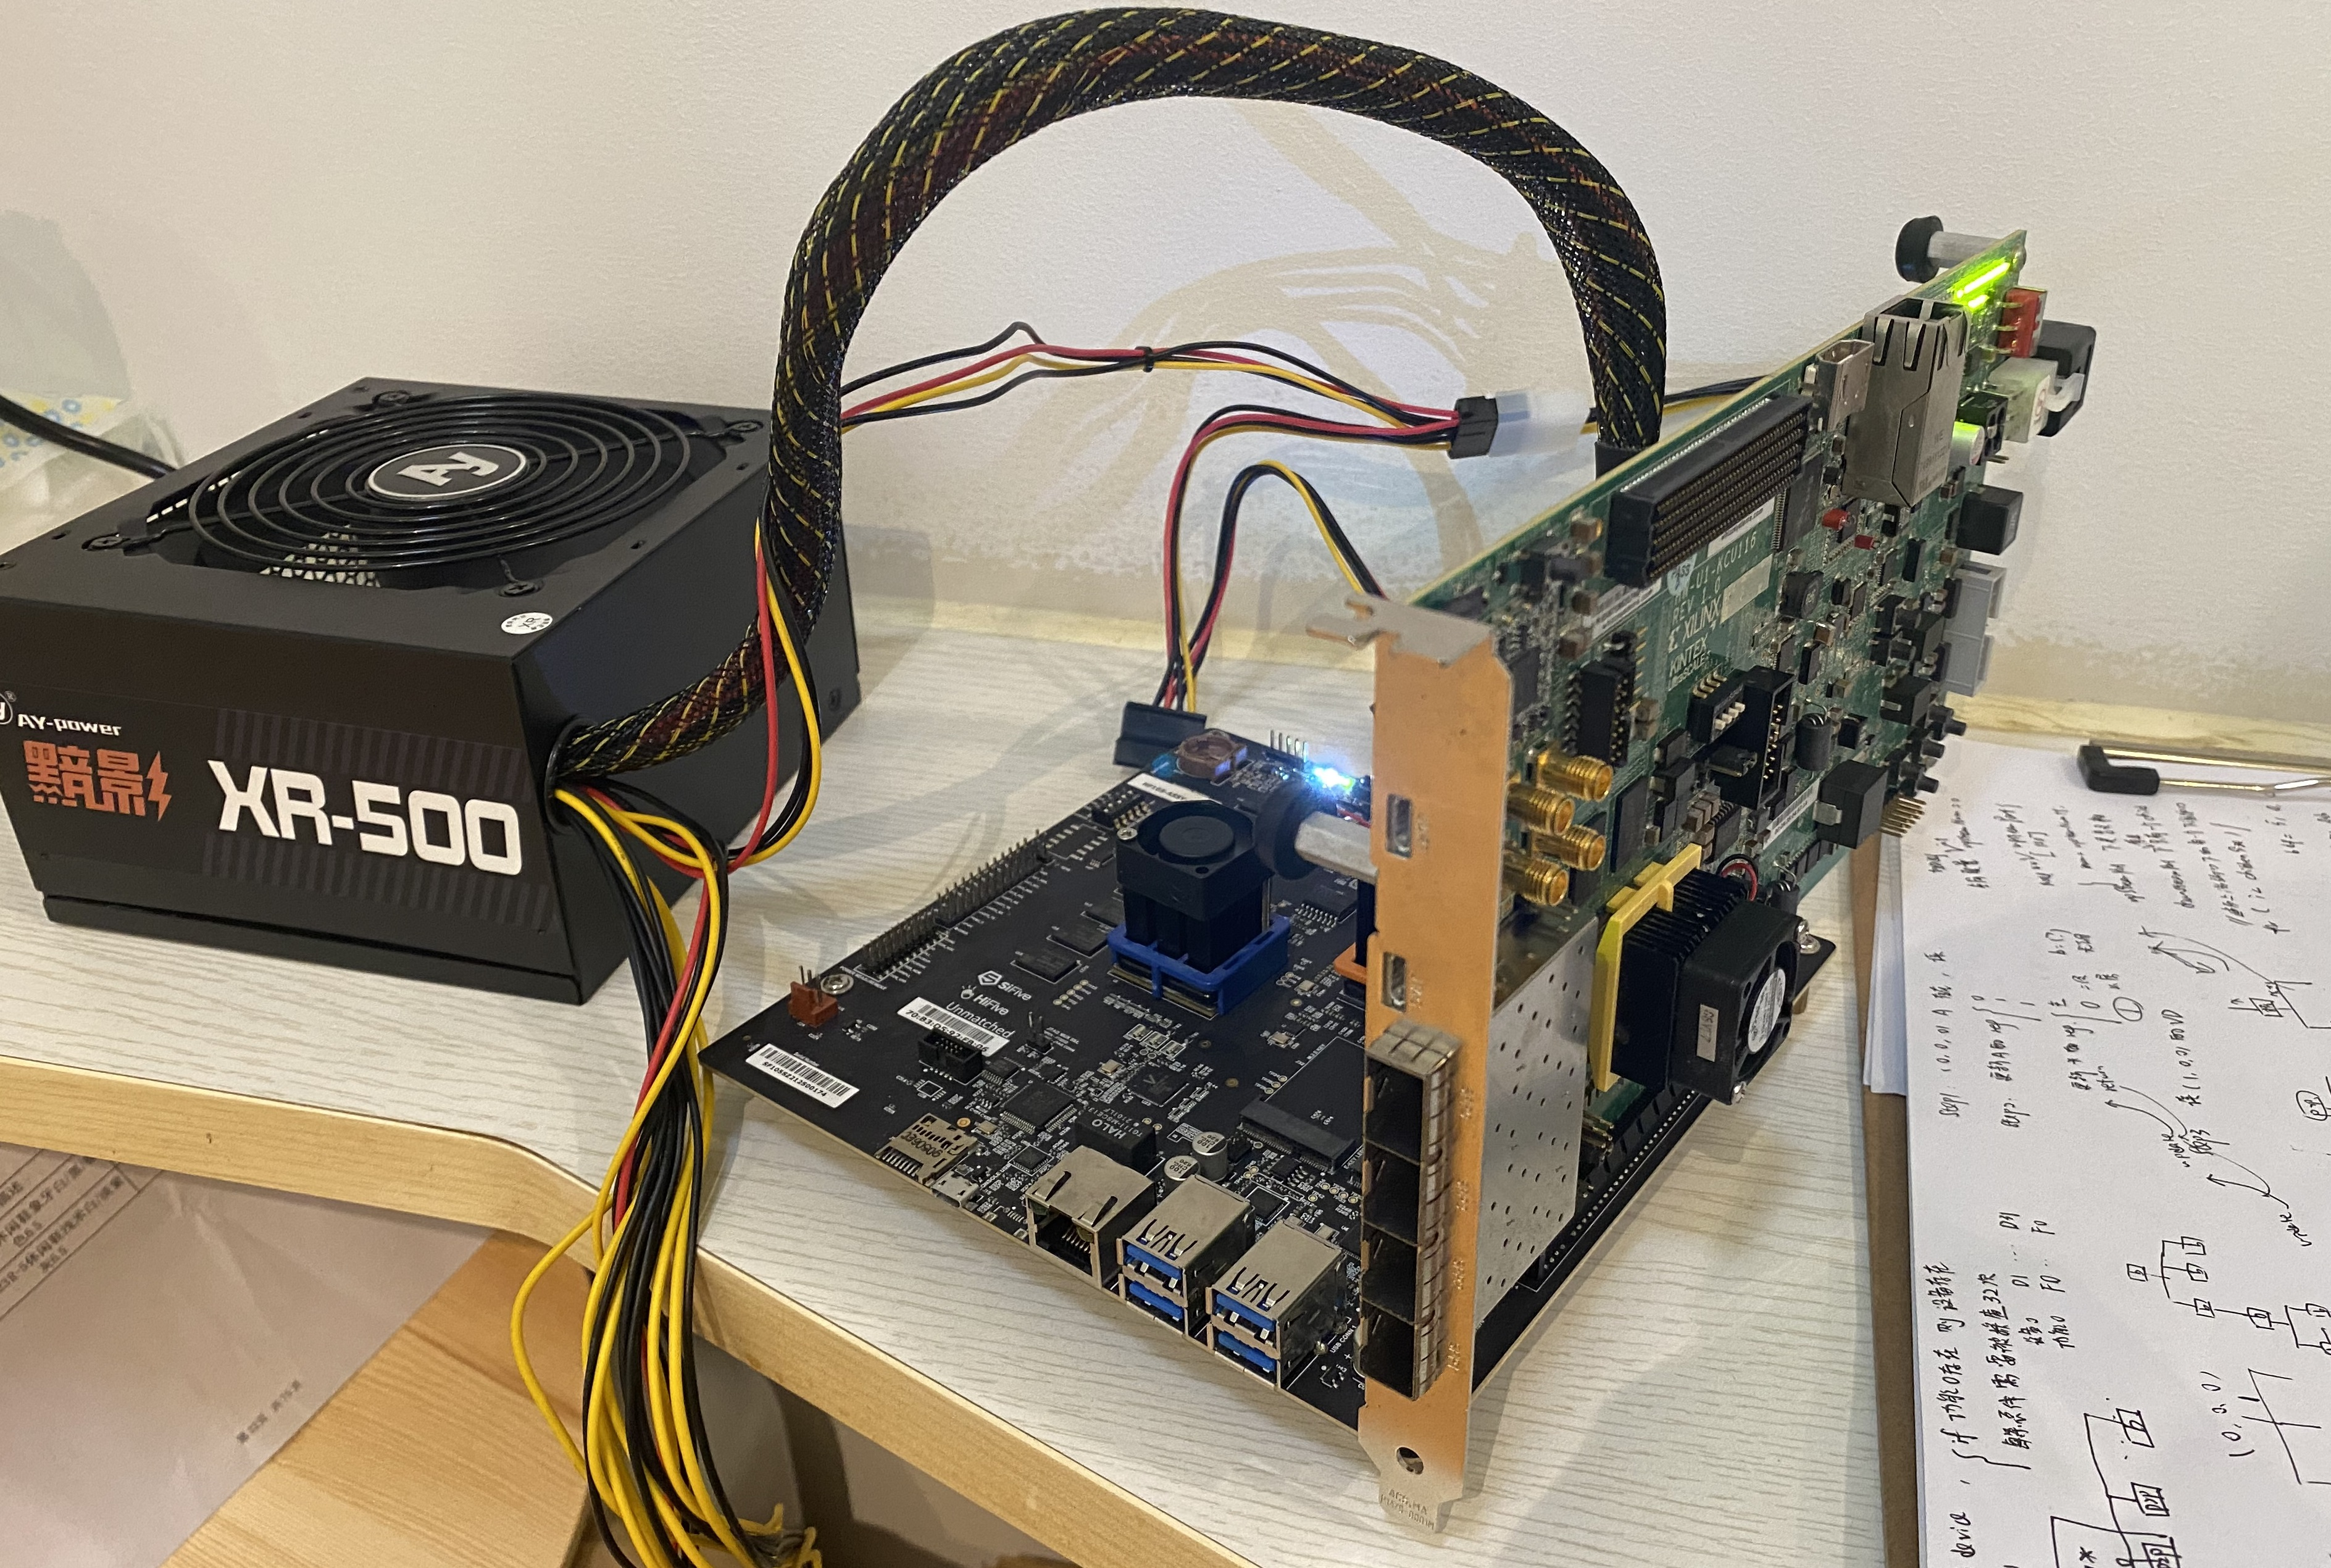
\includegraphics[scale=0.075]{./figs/pcie-tb.jpg}
    \end{figure}
\end{frame}

\begin{frame}
    \frametitle{攻击测试演示}
    在HiFive Unmatched单板计算机上的Linux操作系统中运行测试目标程序
    “hello”,其中存储的秘密数据为“Hellp”字符串。
    \begin{figure}[ht]
        \centering
        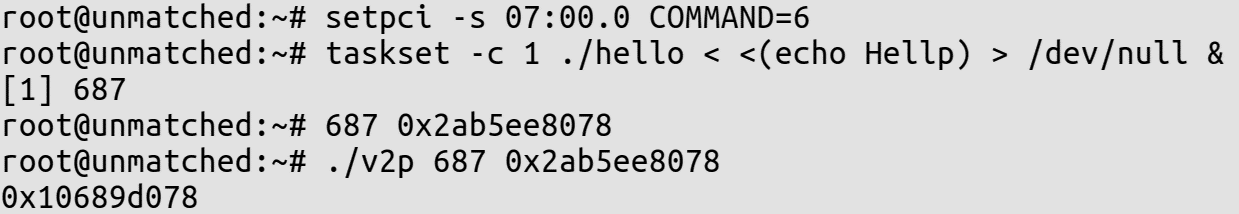
\includegraphics[width=\textwidth]{../paper/figs/unmatched.png}
    \end{figure}
    上位机通过Vivado向PCIe Endpoint发送读取指令,可见返回值在ASCII编码下为
    H(0x48) e(0x65) l(0x6c) l(0x6c) p(0x70),成功读取到了秘密数据。
    \begin{figure}[ht]
        \centering
        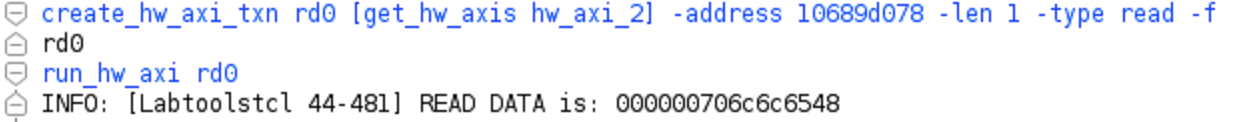
\includegraphics[width=\textwidth]{../paper/figs/vivado.png}
    \end{figure}
\end{frame}




\section{研究总结}

\begin{frame}{}
    \centering
    \Huge\bfseries\textcolor{xmucolor}{研究总结}
\end{frame}

\subsection{攻击方案对比}
\begin{frame}
\frametitle{攻击方案对比}
\begin{table}
    \begin{tabular}{ccccc}
        \toprule
        攻击方式 & 攻击目标 & 物理接触 & 特制硬件 & 实施难易 \\
        \midrule
        FireWire DMA\cite{becher2005firewire} & PC、服务器 & 是 & 是 & 难 \\
        DPA\cite{kocher1999differential} & 嵌入式 & 是 & 是 & 较难 \\
        Acoustic\cite{acoustic} & PC、便携、嵌入式 & 否 & 否 & 中 \\
        Meltdown\cite{lipp_meltdown_2018} & PC、服务器、便携 & 否 & 否 & 易,已修复 \\
        \textbf{本文微架构攻击} & \textbf{PC、服务器、便携} & \textbf{否} & \textbf{否} & \textbf{易} \\
        \textbf{本文系统攻击} & \textbf{PC、服务器} & \textbf{否} & \textbf{否} & \textbf{易} \\
        \bottomrule
    \end{tabular}
\end{table}
\end{frame}

\subsection{后续工作}
\begin{frame}
\frametitle{后续工作}
    \begin{itemize}
        \setlength\itemsep{1em}
        \large
        \item 将高速缓存Evict算法以及Spectre攻击方案移植到香山处理器硬件上验证,
        借助硬件更高的性能完善统计算法,实现更准确的存储器内容读取;
        \item 尝试通过控制GPU的DMA引擎,实现更加普遍的PCIe DMA攻击方案。
    \end{itemize}
\end{frame}


\nocite{*}

\begin{frame}[t,allowframebreaks]
    \frametitle{参考文献}
    \printbibliography[title={参考文献}]
\end{frame}

%------------------------------------------------

\section{}
\begin{frame}{}
    \centering
    \Huge\bfseries\textcolor{xmucolor}{Q\&A}
\end{frame}

\begin{frame}{}
    \centering
    \Huge\bfseries\textcolor{xmucolor}{Thanks!}
\end{frame}

%----------------------------------------------------------------------------------------

\end{document}
